\chaptertitle{11}{基金定投，什么时候卖出}

\setcounter{figure}{0}\setcounter{table}{0}
\subsection{止盈的三种思路}
我们前面介绍了很多优秀的指数基金，也介绍了定投指数基金和增强定投收益的做法。但是还有一个很重要的环节，那就是指数基金的卖出。

俗话说，会买的是徒弟，会卖的是师傅。那关于定投指数基金，该如何卖出呢？

这里的卖出，也被称为“止盈”。关于止盈的操作，有很多不同的思路和方法，最常用的思路有三种。

第一种思路，是投资者从自身收益角度考虑来止盈。

第二种思路，是投资者从投资品种的价值角度考虑来止盈。

第三种思路，是不止盈，低估时买入指数基金，长期持有，依靠基金的分红获取现金流。

最常见的止盈卖出方法，就是以上三种。其实三种方法都有道理，但适用范围是有区别的。

\subsection{按照收益率来止盈，赚多少才能卖}
{\heiti 从收益率角度来考虑止盈}

从收益率角度来考虑止盈，是最常见的基金止盈策略。

这种思路很简单，就是坚持定投指数基金，当看到自己持有的某只基金的收益率达到了设定的收益率，就可以开始卖出止盈。

比如说我们定投沪深300指数基金，当我们看到这只基金的账面收益率达到了我们设定的收益率，如20\%，就可以赎回持有的这只沪深300指数基金，完成投资。

很明显，这种止盈方法，对止盈收益率的设定是非常重要的。

（1）不能太频繁止盈。

因为指数基金包括股票基金，短期买入卖出，赎回费还是比较高的。

我们前面介绍过，指数基金如果持有不到7天就赎回，会有一个惩罚性的赎回费率1.5\%，大大影响投资者的收益。持有超过7天后，大部分指数基金赎回费率是0.5\%。大部分基金继续持有超过2～3年，赎回费免除。

假如说我们设定赚5\%就止盈，同时赎回费率为0.5\%，赎回后再投资其他品种，合计交易成本高达收益的10\%。我们赚到的钱的10\%，都作为费用交给基金平台和基金公司了。反复几次，那收益会大打折扣，很不划算。

（2）止盈的收益率设置得不能太低。

这个止盈的收益率，也不适合设置得太低，否则牛市时赚不了多少钱就止盈，比较浪费。比如说大牛市，可能一轮牛市上涨会超过200\%，如果我们赚了8\%就止盈，那对牛市就比较浪费。

设定止盈收益率时，有一个比较常用的数字：30\%。

{\heiti 赚了30\%就卖出，为何要这样设定}

这个数字是怎么来的呢？

还真不是拍脑袋想出来的。这个止盈的收益率，在A股的一类品种应用很长的时间了，那就是可转债。

什么是可转债呢？

可转债本质上是一类债券品种。债券有约定期限（比如说5年期）、约定利率（比如说每年支付利息多少元），持有这只债券，平时会获得利息，到期了能拿回本金。

可转债也是这样一种债券，不过它增加了一个功能：在到期之前，可以以某一个价格，转换成对应的上市公司股票。这个功能是可转债相对一般债券最大的一个不同点。

这个转股价通常是固定的。试想一下，如果可转债对应的股票价格大涨了，可转债仍然能以较低的价格转换成股票，那这个可转债是很值钱的。于是这个可转债的价格也会随着正股的价格而上涨。

如果对应股票的价格暴跌了呢？可转债也会随着下跌，但是这个下跌是有极限的。因为可转债毕竟是一种债券，它到期了是可以兑付本金的，所以可转债下跌是有保底的。

可转债还有一个很省心的地方：自带止盈策略。

大多数可转债，会有一个强制赎回条款：如果股价在一段时间里，高于设定好的一个值（通常为转股价的130\%），那么上市公司有权按照一个约定价格赎回全部可转债。

可转债发行上市的时候，通常是100元的面值。换句话说，以100元的面值买入的可转债，如果涨了30\%，差不多就要准备卖出止盈了，否则会被公司强制赎回。

实际上牛市疯狂的时候，甚至可转债会在强制赎回执行之前，短期涨到超过130元。

也正是因为这一点，每次牛市的时候，市场上的可转债基本上剩不下几只了。这也是它的一个缺点：并不是一个长期持续的资产种类，只是阶段性地出现投资机会。

换句话说，可转债自带一个“30\%收益率止盈”的策略。

实际上，如果投资可转债，收益率通常比30\%的收益率高。因为可转债上市后，单价很多时候会到90多元，甚至80多元。从90元上涨到130元，收益率上涨是接近45\%的。而且很多可转债会涨到130元以上。

不过总体来看，如果在可转债上市的时候投资它，按照默认的规则，最后对应30\%的收益率止盈。

发行可转债的公司，是希望可转债转换成股票的。因为债券要还本金，但是转换成股票之后，公司就不用拿出这笔现金了。

所以公司在发行可转债的时候，是有动力做好研究、精心设计好规则，让可转债尽量能到期转股。

绝大部分可转债，设计的年限是5年。

最后大部分可转债，都成功转股了，没转股的是少数。而且通常不到5年，2～3年就实现了。

所以可转债“30\%收益率止盈”的策略，是一个很有效的止盈策略。平均2～3年就可以止盈一次。

可转债虽然是一种债券，但是它的投资收益和风险特征，跟指数基金中很多品种比较相似。可转债涨跌区间跟指数基金高度重合。所以如果套用到宽基指数基金上，“30\%收益率止盈”的策略在原理上是可行的，2～3年就可以大概率遇到一次“30\%收益率止盈”的机会。

{\heiti 收益率止盈的缺点}

不过这种止盈策略，也有如下缺点。

（1）不同投资者开始投资的阶段不同，有的投资者是熊市很低估的时候开始投资，有的投资者可能涨了一截才开始投资。这就会出现“有人辞官归故里，有人星夜赶考场”的情况。有的人止盈了，有的人才开始投资。所以这种止盈，只能是大家根据自己的收益情况，判断是不是需要这样止盈。

（2）大牛市疯狂阶段的涨幅会更高，投资者会缺失一些收益。

（3）比较适合波动大的品种。因为只需要赚30\%就止盈，对短期波动大的品种使用这类策略更适合，例如中证500指数基金等。这类品种波动大，更容易触发止盈。

这种止盈策略，比较适合可能在未来2～3年内要用到这笔资金的朋友。

按照“定投低估指数基金，30\%收益率止盈”，在2～3年内实现止盈获利是大概率的。

\subsection{按照估值来止盈}
第二种止盈的思路，是按照估值来止盈。

指数基金有自己的投资价值。如果价格大幅低于价值，也就是我们所说的低估。如果价格大幅高于价值，也就是我们所说的高估。我们在低估区域定投指数基金，就是买入价格低于其应有价值的指数基金。那反过来，如果要我们卖出，也是因为价格大幅高于价值。这也是我们目前经常用到的一种止盈方法。

这种方法的投资周期，要比按照“30\%收益率止盈”策略更长。因为一般在大牛市的中后期，才会到高估区域，例如2007年、2015年大牛市，其他时间估值是达不到很高的位置的。大牛市通常7～10年一轮，所以使用这种投资方式时，中间需要有耐心持有。

这种止盈方式的优缺点也很明显。

{\heiti 估值止盈的优点}

第一个优点，是在牛市收益高。

通常从低估到正常估值，从正常估值到高估，每一个区域都有30\%～40\%的涨幅。

到了高估区域，如果遇到像2006—2007年那种大牛市，涨幅很惊人。所以这种止盈方法，能在牛市获得很高的收益。

第二个优点，是投资者可以比较长地享受到投资品种本身盈利上涨带来的收益。

有的朋友会担心，牛市那么长时间才来一次，如果牛市没来，岂不是很长时间里不赚钱？其实不用担心的。

拆分一下指数基金的净值：

{\kaishu 指数基金净值=市盈率×盈利+分红}

对于有的指数基金来说，自身盈利增长是非常不错的。每年盈利增长都有10\%～20\%。例如我们前面介绍过的策略加权指数基金，如红利、基本面、价值、低波动等，以及长期优秀的行业指数基金，如消费、医药、中概互联等。这些品种的长期盈利增长不错。假如说在7年时间里牛市没有来，估值始终在正常估值，这些指数基金的净值也是涨幅不错的。

例如，2012年，A股的中证红利指数、医药100指数的市盈率，跟2019年年初的估值是差不多的。但是这段时间里，中证红利指数基金的净值和医药100指数基金的净值，均上涨超过120\%。

市盈率不变，净值上涨120\%，主要就是盈利增长和分红积累带来的。

实际上，对很多盈利增长不错的品种来说，不适合使用“30\%收益率止盈”的策略。

这些盈利增长不错的品种，即使估值保持一个位置不变，依靠盈利增长，净值每年都平均上涨15\%～20\%。

例如，很多股民熟悉的大牛股都是这种类型：长期盈利增长不错，可能10年时间里会上涨几倍甚至十几倍。

仅仅赚30\%就止盈太可惜了，这也就是指数背后公司一两年的盈利增长。

试想一下，在涨了几百倍的茅台和腾讯上，只赚了30\%就止盈卖出，真是暴殄天物。

{\heiti 估值止盈的缺点}

第一个缺点，是投资者需要非常有耐心。

按照30\%收益率止盈，通常2～3年就能遇到一次。但是按照高估来止盈，必须要有大牛市，那就得7年甚至10年才能等到。在牛市来之前，投资者需要耐心持有，享受背后公司的盈利上涨，面对中间涨涨跌跌的波段需要不为所动，这不是所有投资者都可以坚持下来的。如果坚持下来，收益会很丰厚。

第二个缺点，这种策略对指数基金的品种有要求。

如果指数基金背后公司的盈利增长速度本身比较慢，那就不适合用这种止盈的思路了。目前适合第二种止盈思路的，主要是两类：一类是优秀的宽基指数基金，特别是策略加权指数基金，如红利、基本面、价值、低波动等；另一类是优秀的行业指数基金；如消费、医药、中概互联等。

{\heiti 按估值止盈的优化：梯度止盈}

我们前面介绍过，在定投指数基金的时候，我们会应用定期不定额的方法。指数基金越低估，我们买入越多。

当指数基金估值进入高估区域，我们卖出指数基金，其实也可以使用同样的方式。只不过是反过来，进入高估区域后，我们把手里的指数基金分成多份，估值越高，卖出的比例也越高。

这种分批卖出、按照估值调整卖出金额的止盈方式，也被称为“梯度止盈”。

比如说一只指数基金，在20倍市盈率以上进入高估区域。进入高估区域的时候，我们持有这只指数基金1万份。当指数基金达到20倍市盈率时，我们卖出10\%的基金份额。下个月，当指数基金达到24倍市盈率时，我们卖出10\%×（24/20）\textsuperscript{2} =14.4\%的基金份额。估值越高，我们卖出的比例越高。

这种卖出方式的好处是，防止在牛市初期就把指数基金全部卖出。因为一次大牛市，可能市场整体涨幅会很高，如果刚进入高估就卖出了，后面的收益会缺失。不过风险是，有可能牛市结束了，还没有卖完。

不过相比一次性进入高估止盈来说，梯度止盈可以把卖出门槛降低一些，更容易达到卖出的条件。跟定期不定额买入相配合，也是不错的技巧。

\subsection{不止盈，长期持有}
{\heiti 长期持有的投资策略}

第三种思路，是不止盈，也就是买入低估的指数基金，然后长期持有，以分红的形式获取现金流。

首先长期持有不卖出，靠分红获得收益，这样的投资策略是存在的。而且“股神”巴菲特和“指数基金之父”约翰·博格都提倡过这种投资方法。

约翰·博格认为，如果客户的收入需求和指数基金的股息分红、利息收入等相匹配，那就没有比简单的坚持到底更好的投资策略了。（2000年）

换句话说，也就是长期持有，依靠每年的现金分红来获取现金流，满足生活所需。

当然，这样做要求投资者有一个足够强壮的心脏。遇到股市大幅波动的时候，能够坚持下来。

{\heiti 长期持有不卖出的收益}

这种投资策略的收益如何呢？

在投资指数基金的过程中，投资者能收获两种收益：一种是资本利得收益（净值上涨的收益），另一种是分红收益。

在持有指数基金的时候，基金净值会长期上涨，但是因为不卖出，这部分收益短期内不会兑现，所以主要是每年收获现金分红收益。

因为指数基金自身具备长生不老的特征，只要背后公司正常经营，这些公司的盈利就是长期上涨的。现金分红作为盈利的一部分，也会随之长期上涨。指数基金就变成了一个“利息收益不断上涨”的超长期理财产品。

我们以盈富基金为例。

盈富基金的分红非常稳定，它的每份基金历年分红记录如下，具体如图 \ref{fig:11-1} 所示。

{\kaishu 2011年全年：0.63港元。}

{\kaishu 2012年全年：0.66港元。}

{\kaishu 2013年全年：0.73港元。}

{\kaishu 2014年全年：0.84港元。}

{\kaishu 2015年全年：0.81港元。}

{\kaishu 2016年全年：0.78港元。}

{\kaishu 2017年全年：0.93港元。}

{\kaishu 2018年全年：0.95港元。}

如图 \ref{fig:11-1} 所示，我们可以看到盈富基金每年的分红是长期增长的。当然，长期增长不等于每年都增长，偶尔一两年会下降一些。

\begin{figure}[htbp]
\centering
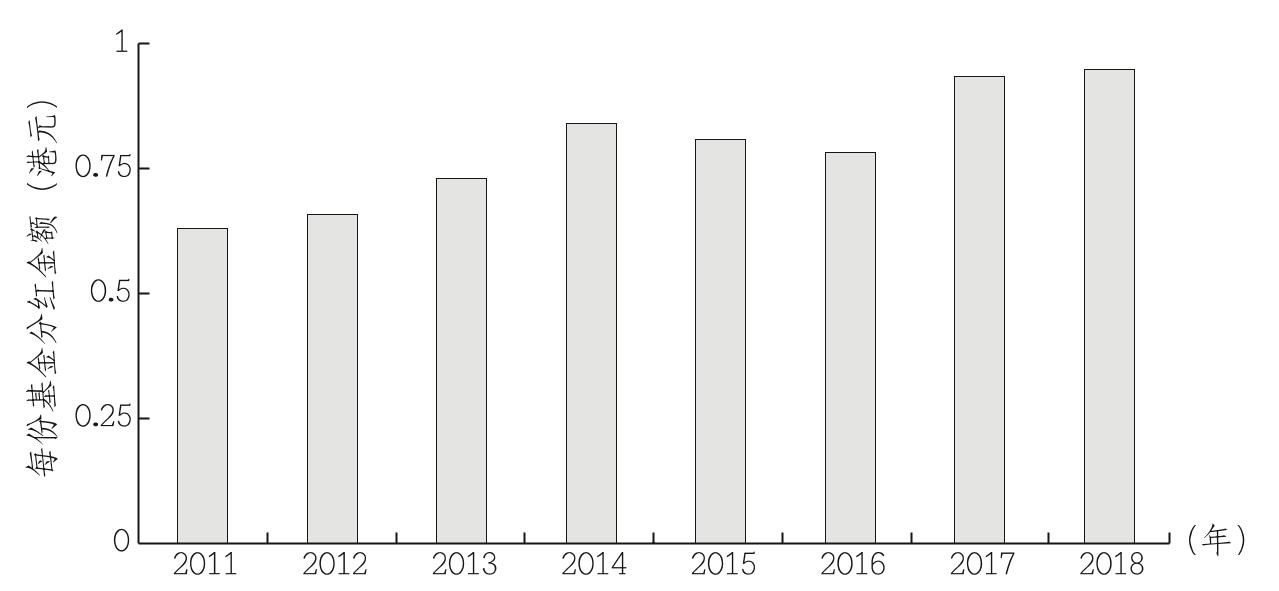
\includegraphics[width=\textwidth,height=0.82\textheight,keepaspectratio]{figure/图11.1.png}
\caption{盈富基金每份基金分红}\label{fig:11-1}
\end{figure}

对指数基金来说，基金分红的主要来源是背后公司的分红。

公司每年赚取盈利的30\%～40\%，会以现金分红的形式发放给股票持有者。指数基金持有股票，也会收到这些现金分红。基金攒一攒，会在某一天以基金分红的形式发放给基金持有者。

这就是指数基金分红的由来。

一般的股票基金分红，可能是基金经理卖出股票，获得现金，然后分红。不过指数基金分红很少是因为卖出股票，主要是因为成份股的分红。这是两者的区别。

我们前面提到过，指数背后公司的盈利是长期上涨的，分红是盈利的30\%～40\%，自然也是长期上涨的。

所以，盈富基金每年分红的金额也是长期上涨的。只不过这个长期上涨不是每年都上涨。遇到像2008年金融危机等情况，可能短期内公司盈利也会受到影响，需要一段时间后才恢复重新上涨。

假如说我们持有10万股盈富基金，在2003年会收到4.1万港元，之后每年都会收到，并且越来越高，到了2018年会收到9.5万港元。未来还会越来越高。

这就是不卖出指数基金的投资方法：指数基金长生不老，我们一直持有，获得现金流。

此时，指数基金就变成了一个永续理财产品。这个理财产品没有到期时间，每年支付一次分红。

{\heiti 长期持有的条件}

这种投资方法要注意以下几点。

（1）适合股息率高的指数基金。

这种方法，适合股息率高、分红多的指数基金。

通常，指数基金分红能不能长期持续，看的是股息率。如果一个指数的股息率长期比较高且稳定，是适合使用这种方法的。主要是大盘宽基指数基金，如上证50、沪深300、恒生、H股，以及红利类策略加权指数基金，如中证红利、红利机会等。

（2）长期分红收益与初始买入时的股息率关系较大。

很明显，这种投资方式跟开始投资时的股息率关系很大。

如果开始投资的时候股息率高达5\%，那第一年现金分红收益率就有5\%。投入100万元，第一年分红就是有5万元。之后每年分红会越来越多。到了第20年，估计一年分红就有48万元。20年能收到的总分红是360万元左右。

但是如果开始投资的时候，股息率只有2\%（例如2015年牛市顶峰的时候），那以这个估值买入100万元，第一年分红只有2万元，第20年的分红大约是19万元，20年收到的总分红约144万元。

20年后，一个360万元，一个144万元，差距还是非常大的。

所以用这种不卖出的思路，一定要在指数基金股息率高的时候投资。

通常对宽基指数基金来说，如果股息率超过4\%，未来的分红收益率不错，超过5\%就是比较少见的好机会了。但是如果2\%都不到，那就要小心。

通常股息率比较高的时候，往往也是大熊市指数基金处于低估的时候，也暗含了低估值投资的理念。所以如果打算长期持有获取分红收益，一定要在股息率比较高的时候再买入。

\subsection{不同止盈方法，适合不同的品种和需求}
至此，我们就介绍完三种不同的止盈方法了。其实聪明的投资者看完这一章，就会明白为何会有三种不同的止盈方式了。

因为影响指数基金收益最大的三个因素，就是估值变化、盈利的增长、分红的积累。三种止盈方式，其实就是基于这三个不同因素，只不过侧重点不同。

第一种止盈方式，是按照收益率止盈，通常喜欢的是暴涨暴跌的品种。这类品种一般周期性比较强，估值变化非常大，而自身的盈利增长和分红通常不太高。所以定投这种波动大、周期性强、估值变化剧烈的品种，按照收益率止盈效率会更高。通常2～3年就可以止盈一次。代表就是证券、能源等周期性比较强的行业。

第二种止盈方式，是按照估值止盈，高估时卖出。使用这种止盈方式，投资者会长时间持有指数基金，通常在一轮牛熊市里都持有。这个过程中，如果指数基金自身的盈利增长高，那最后叠加牛市估值的上涨，带来的总收益是非常惊人的。这类品种不应该按照收益率止盈，否则浪费了背后公司的盈利增长。代表就是优秀的宽基指数基金，如红利、基本面、价值、低波动等。另外还有优秀的行业指数基金，如消费、医药、中概互联等。大牛市没来时，低估买入，持有它们，也会有很不错的收益。通常是7～10年止盈一次。

第三种止盈方式，是不止盈，长期持有拿分红。只要买入时的股息率比较高，长期来看指数基金提供的分红现金流也会比较稳定。依靠分红现金流能满足日常生活的需求，投资者也就不需要再揪心股票市场的涨涨跌跌了。代表就是股息率高的宽基指数基金，如上证50、沪深300、恒生、H股、标普500等，以及高股息率的红利类指数基金。

通常一个投资品种，只适合一到两种止盈方式，无法三者兼顾。

比如说红利类品种，用第二、第三种止盈方式都可以，但是第一种就不太合适。因为高股息率的红利类品种通常波动都不太大，牛市弹性不高。“30\%收益率止盈”策略，更适合波动大的品种，容易达成止盈的条件。

而证券行业，适合使用第一、第二种方式，但第三种方式不合适。因为证券行业盈利不稳定，分红很难稳定，长期持有它也没有分红现金流。

如果一个品种盈利不稳定、估值变化大，最好用收益率止盈方法。

如果一个品种盈利增长比较稳定，那适合低估时买入，长期持有，耐心等高估。

如果一个品种盈利稳定，分红良好，可以在低估、高股息率的时候买入，长期持有获取分红。

品种的特征，决定了止盈的特征。

{\heiti 投资者笔记}

\begin{itemize}
\item {\kaishu 投资基金的卖出思路有三种：按照收益率来止盈，按照估值来止盈，以及长期持有不卖出。}
\item {\kaishu 不同的止盈方法，适合不同的投资品种和投资需求。}
\end{itemize}

